\chapter{Geometria}

\section{Planimetria}

\begin{example}
	Pozemok má pôdorys v tvare kosodĺžnika. Na pláne s mierkou 1 : 5 000 má jedna zo strán
	kosodĺžnika dĺžku 9 cm a priľahlá výška má 7 cm. Koľko hektárov zaberá pozemok
	v skutočnosti? Výsledok uveď s presnosťou na stotiny.
	
	\begin{center}
		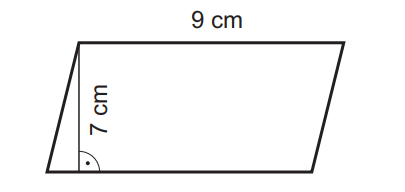
\includegraphics{assets/pozemok.png}
	\end{center}
\end{example}

\begin{example}
	Vypočítaj v stupňoch veľkosť ostrého uhla, ktorý zvierajú ručičky hodín o pol šiestej.
	
	\begin{center}
		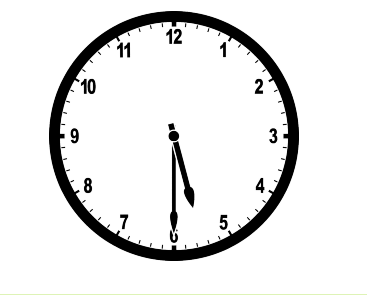
\includegraphics{assets/hodiny.png}
	\end{center}
\end{example}

\begin{example}
	Osemuholník ABCDEFGH sa skladá z ôsmich zhodných trojuholníkov. Obsah tohto
	osemuholníka je 33,6 $cm^2$. Vypočítaj obsah časti vyfarbenej tmavou farbou. Výsledok uveďv $cm^2$.
	
	\begin{center}
		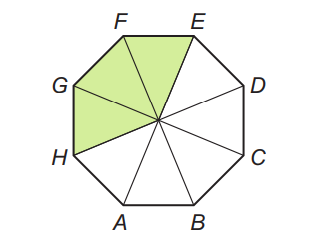
\includegraphics{assets/osemuholnik.png}
	\end{center}
\end{example}

\begin{example}
	Priamka k je rovnobežná s priamkou l. Priamka m je kolmá na priamku k. 
	Priesečník priamok k a m označme A. Priesečník priamok l a m označme B.
	Priamka n je rôznobežná so všetkými predchádzajúcimi priamkami a priesečník priamok m a n neleží na úsečke AB. Priesečník priamok l a n označme C. Priesečník priamok k a n označme D. Na základe toho, čo vieme o vzájomnej polohe uvedených priamok, je štvoruholník ABCD
	určite aký útvar?
\end{example}

\begin{example}
	V štvorcovej sieti so stranou štvorca dlhou 1 cm sú znázornené 4 štvoruholníky, medzi ktorými je aj pravouhlý lichobežník. V ktorej možnosti je správne uvedený jeho obsah?
	
	\begin{center}
		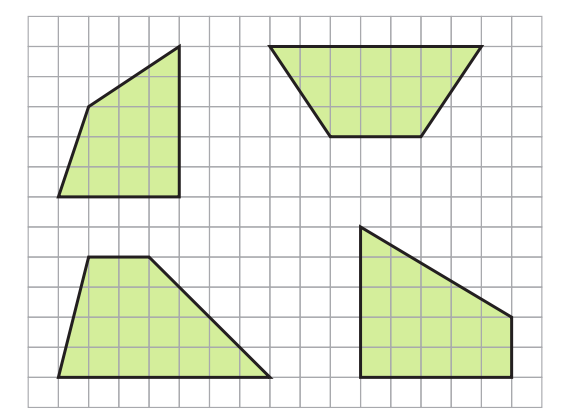
\includegraphics{assets/lichobezniky.png}
	\end{center}
	
	\begin{enumerate}
		\item $18 ~ cm^2$
		\item $17.5 ~ cm^2$
		\item $15 ~ cm^2$
		\item $13.5 ~ cm^2$
	\end{enumerate}
\end{example}

\begin{example}
	Vypočítaj obsah pravouhlého trojuholníka ABC, ak poznáš obsah štvorca nad preponou BC a tiež obsah štvorca nad odvesnou AC. 
	
	\begin{center}
		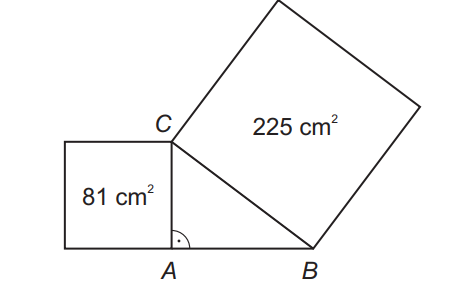
\includegraphics{assets/pravouhly.png}
	\end{center}
\end{example}

\begin{example}
	\begin{center}
		
\includegraphics{assets/uhol_zadanie.png}
		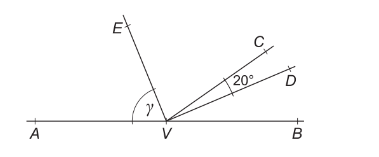
\includegraphics{assets/uhol.png}
	\end{center}
\end{example}

\begin{example}
	
	\begin{center}
		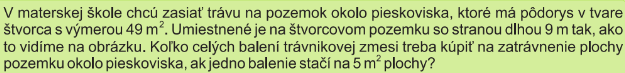
\includegraphics{assets/pieskovisko_zadanie.png}\\
		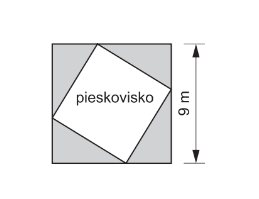
\includegraphics{assets/pieskovisko.png}
	\end{center}
\end{example}

\begin{center}
	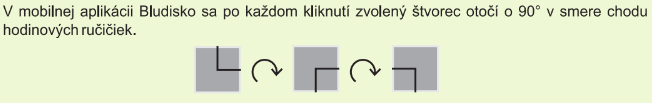
\includegraphics{assets/bludisko_zadanie.png}
\end{center}

\begin{example}
	1. príklad k bludisku.\\
	\begin{center}
		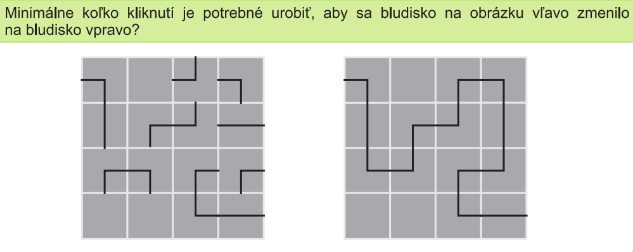
\includegraphics{assets/bludisko1.png}
	\end{center}
\end{example}

\begin{example}
	2. príklad k bludisku. \\
	
	\begin{center}
		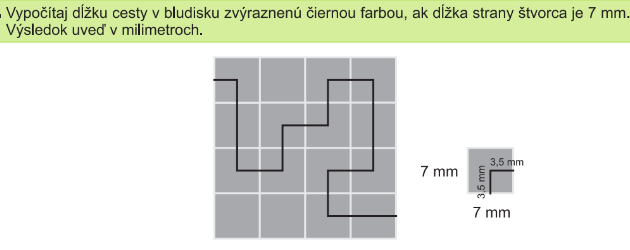
\includegraphics{assets/bludisko2.png}
	\end{center}
\end{example}

\begin{example}
	\begin{center}
		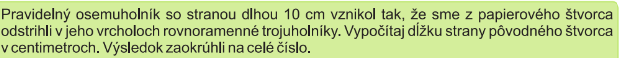
\includegraphics{assets/osemuholnik2_zadanie.png}
		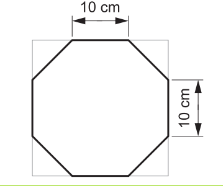
\includegraphics{assets/osemuholnik2.png}
	\end{center}
\end{example}


	
\begin{center}
	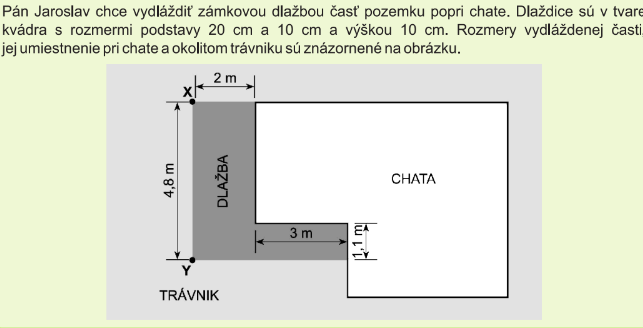
\includegraphics{assets/chata.png}
\end{center}

\begin{example}
	1. príklad k chate.
	\begin{center}
		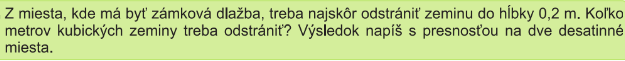
\includegraphics{assets/chata1.png}
	\end{center}
\end{example}

\begin{example}
	2. príklad k chate.
	
	\begin{center}
		
\includegraphics{assets/chata2.png}
	\end{center}
\end{example}

\begin{example}
	Dlažba:
	
	\begin{center}
		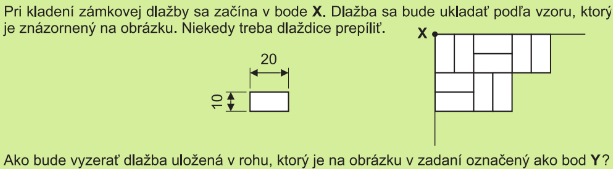
\includegraphics{assets/dlazba_zadanie.png}
		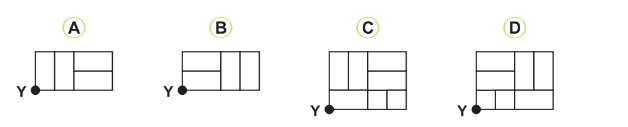
\includegraphics{assets/dlazba_moznosti.png}
	\end{center}
\end{example}

\begin{example}
	Kocka:
	\begin{center}
		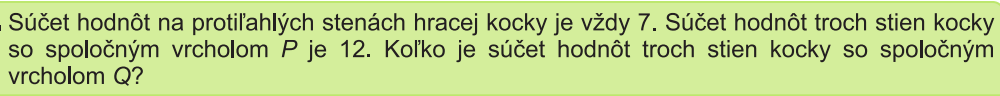
\includegraphics[width=\linewidth]{assets/kocka_zadanie.png}
		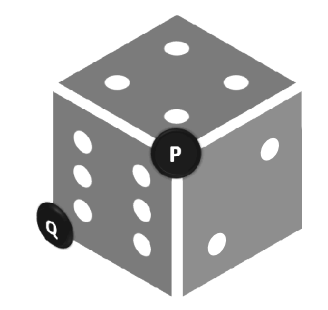
\includegraphics{assets/kocka.png}
	\end{center}
\end{example}

\begin{example}
	Kruhy:
	
	\begin{center}
		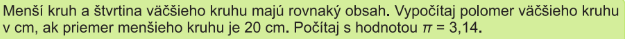
\includegraphics{assets/kruhy_zadanie.png}
		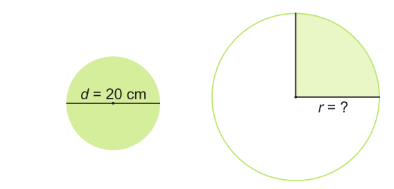
\includegraphics{assets/kruhy.png}
	\end{center}
\end{example}

\begin{example}
	Stavby:
	
	\begin{center}
		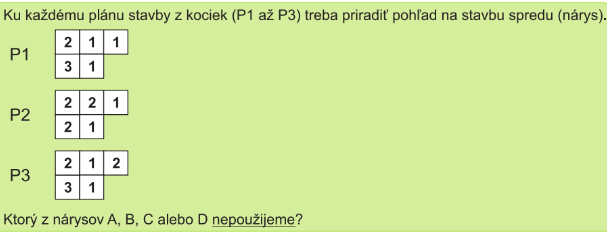
\includegraphics{assets/stavby_zadanie.png}
		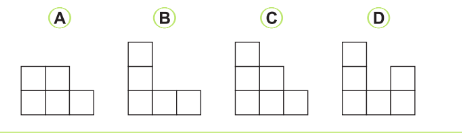
\includegraphics{assets/stavby_moznosti.png}
	\end{center}
\end{example}

\begin{example}
	Kmeň stromu:
	
	\begin{center}
		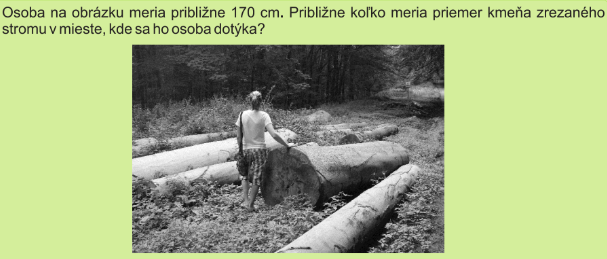
\includegraphics{assets/strom_zadanie.png}
		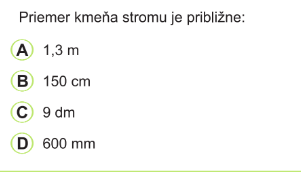
\includegraphics{assets/strom_moznosti.png}
	\end{center}
\end{example}

\begin{example}
	Škatulky:
	
	\begin{center}
		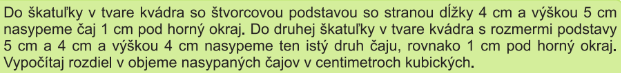
\includegraphics{assets/skatulky_zadanie.png}
		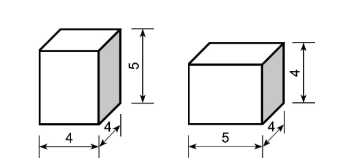
\includegraphics{assets/skatulky.png}
	\end{center}
\end{example}

\begin{example}
	Kontajner:
	
	\begin{center}
		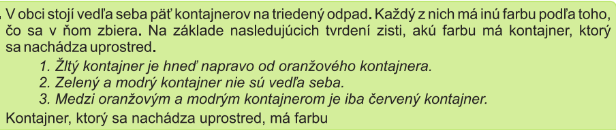
\includegraphics{assets/kontajner_zadanie.png}
		
\includegraphics{assets/kontajner_moznosti.png}
	\end{center}
\end{example}

\begin{example}
	Štvorec:
	
	\begin{center}
		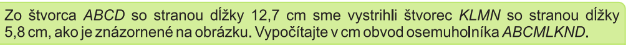
\includegraphics{assets/stvorec_zadanie.png}
		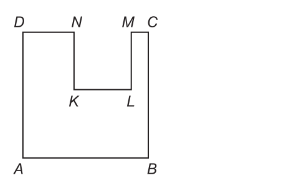
\includegraphics{assets/stvorec.png}
	\end{center}
\end{example}

\begin{example}
	Škatuľka:
	
	\begin{center}
		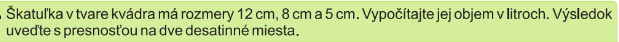
\includegraphics{assets/skatulka.png}
	\end{center}
\end{example}

\begin{example}
	Sud:
	
	\begin{center}
		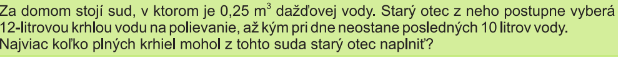
\includegraphics{assets/sud.png}
	\end{center}
\end{example}

\begin{example}
	Danina izba:
	
	\begin{center}
		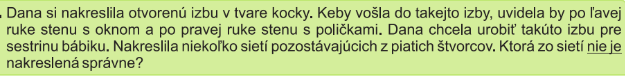
\includegraphics{assets/dana_zadanie.png}
		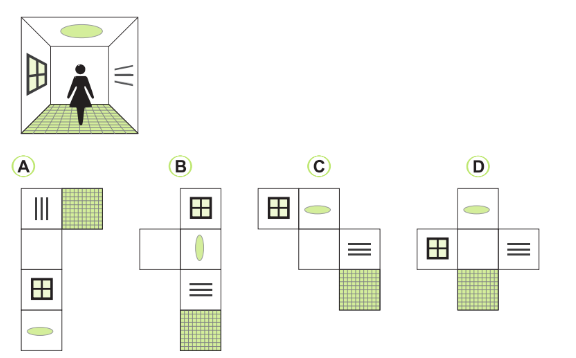
\includegraphics{assets/dana_moznosti.png}
	\end{center}
\end{example}

\begin{example}
	Pán Novák a jeho psy:
	
	\begin{center}
		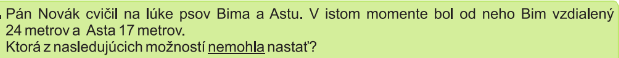
\includegraphics{assets/psy.png}
		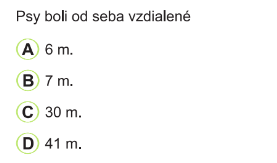
\includegraphics{assets/psy_moznosti.png}
	\end{center}
\end{example}

\begin{example}
	\begin{center}
		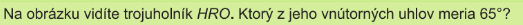
\includegraphics{assets/uhol2_zadanie.png}
		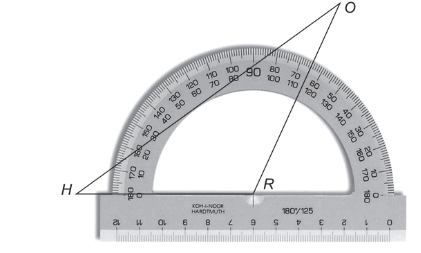
\includegraphics{assets/uhol2.png}
		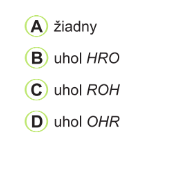
\includegraphics{assets/uhol2_moznosti.png}
	\end{center}
\end{example}

\begin{example}
	\begin{center}
		
\includegraphics{assets/pravouhly2_zadanie.png}
		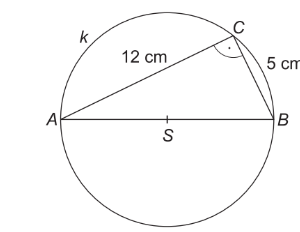
\includegraphics{assets/pravouhly2.png}
	\end{center}
\end{example}

 \begin{example}
 	\begin{center}
 		
\includegraphics{assets/siet_zadanie.png}
 		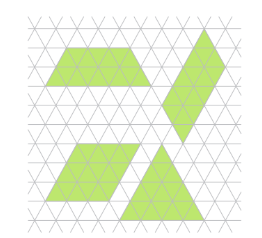
\includegraphics{assets/siet.png}
 	\end{center}
 \end{example}
 
 \begin{example}
 	Strýko Jonatán a heslo:
 	
 	\begin{center}
 		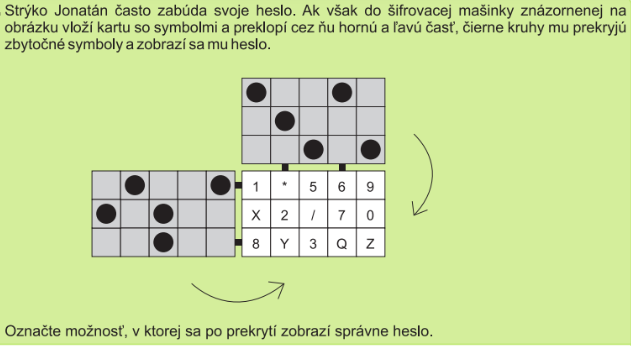
\includegraphics{assets/jonatan_zadanie.png}
 		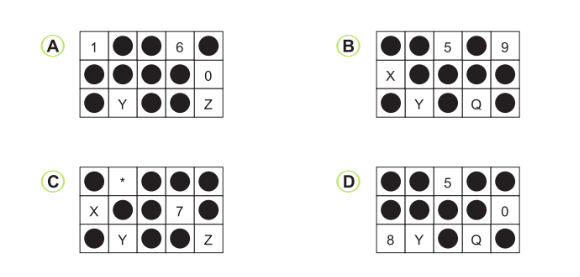
\includegraphics{assets/jonatan_moznosti.png}
 	\end{center}
 \end{example}
 
 \begin{example}
 	\begin{center}
 		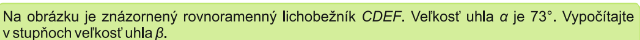
\includegraphics{assets/lichobeznik_zadanie.png}
 		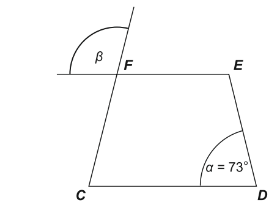
\includegraphics{assets/lichobeznik.png}
 	\end{center}
 \end{example}
 
 \begin{example}
 	\begin{center}
 		\includegraphics{assets/stvorec2.png}
 	\end{center}
 \end{example}
 
 \begin{example}
 	\begin{center}
 		\includegraphics{assets/trojuholnik_zadanie.png}
 		\includegraphics{assets/trojuholnik_rozmery.png}
 		\includegraphics{assets/trojuholnik.png}
 	\end{center}
 \end{example}

\begin{example}
	\begin{center}
		\includegraphics{assets/papier_zadanie.png}
		\includegraphics{assets/papier1.png}
	\end{center}
\end{example}

\begin{center}
	\includegraphics{assets/byty_zadanie.png}
\end{center}

\begin{example}
	\begin{center}
		\includegraphics{assets/byty1.png}
	\end{center}
\end{example}

\begin{example}
	\begin{center}
		\includegraphics{assets/byty2.png}
	\end{center}
\end{example}
 

\section{Stereometria}

\begin{example}
	Zisti, ktoré číslo treba dosadiť za $x$, aby platila rovnosť 2 hl + 30 dl + $x$ $dm^3$ = 206,7 $dm^3$.
\end{example}

\begin{example}
	Koľkokrát má kocka s hranou dlhou 9 dm väčší objem ako kocka s hranou dlhou 3 cm?	
\end{example}

\begin{example}
	Na obrázku je znázornený úložný box v tvare kvádra s rozmermi 42 cm, 24 cm a 24 cm vyplnený zhodnými kockami. Koľko kociek je spolu v úložnom boxe, ak v hornej vrstve vidíme 28 kociek?
	
	\begin{center}
		\includegraphics{assets/box.png}
	\end{center}
	
\end{example}

\textbf{Pracovná doska stola má byť umiestnená v rohu kancelárie. Jej podstava má tvar štvrťkruhu, pričom polomer kruhu je 90 cm. Hrúbka dosky je 2 cm.}

\begin{example}
	Hrany pracovnej dosky sa upravia tak, že sa po celom obvode dosky nažehlí hranovacia páska.
	Koľko centimetrov hranovacej pásky sa spotrebuje na olemovanie jednej pracovnej dosky?
	Počítaj s hodnotou $\pi = 3,14$. Výsledok zaokrúhli na celé centimetre nahor. 
	
	\begin{center}
		\includegraphics{assets/doska1.png}
	\end{center}
\end{example}

\begin{example}
	Pracovné dosky sa vyrezávajú z dosiek s podstavou v tvare štvorca so stranou dĺžky 180 cm.
	Koľko percent tvorí odpad pri vyrezaní štyroch takýchto pracovných dosiek? Počítaj s hodnotou
	$\pi= 3,14$. 
	
	\begin{center}
		\includegraphics{assets/doska2.png}
	\end{center}
\end{example}

\begin{example}
	Na obrázku sú 3 telesá. Hrana kocky je dlhá 3 cm. Kváder má dva rozmery rovnaké ako kocka,
	jeho tretí rozmer je 2-krát dlhší. Valec je rovnako vysoký ako kocka a priemer jeho podstavy
	je 3 cm.
	
	\begin{center}
		\includegraphics{assets/telesa.png}
	\end{center}
	
	Z týchto troch telies možno postaviť rôzne stavby. Predpokladajme, že kváder v stavbe
	je položený ako na obrázku. V nasledujúcich možnostiach sú uvedené pohľady zhora
	na niektoré z týchto stavieb. V ktorej možnosti je pohľad na stavbu z týchto troch telies, ktorá by určite nemohla mať práve dve poschodia?
	
	\begin{center}
		\includegraphics{assets/telesa_moznosti.png}
	\end{center}
\end{example}

\begin{center}
	\includegraphics[width=\linewidth]{assets/zahon.png}
\end{center}

\begin{example}
Koľko centimetrov má výška vrstvy tvorenej substrátom a kompostom, ak pomer výšky tejto
vrstvy a výšky vrstvy konárov je 5 : 8? 
\end{example}

\begin{example}
	V ktorej možnosti je správne uvedený objem vrstvy konárov vo vyvýšenom záhone?
	
	\begin{enumerate}
		\item $54 ~ dm^3$
		\item $5.4 ~ m^3$
		\item $540 ~ l$
		\item $0.54 ~ hl$
	\end{enumerate}
\end{example}

\begin{center}
	\includegraphics{assets/aquapark_zadanie.png}
\end{center}

\begin{example}
	\begin{center}
		\includegraphics{assets/aquapark1.png}
	\end{center}
\end{example}

\begin{example}
	\begin{center}
		\includegraphics{assets/aquapark2.png}
	\end{center}
\end{example}

\begin{example}
	\begin{center}
		\includegraphics{assets/kocka2_zadanie.png}
		\includegraphics{assets/kocka2_moznosti.png}
		\includegraphics{assets/kocka2.png}
	\end{center}
\end{example}



